% The same space, the same data constraint, two ways of choosing within it.
%   left  -- reweighting picks one point of a huge consistent set, by leaning on
%            the distribution the cloud was drawn from.
%   right -- restricting to a family first leaves a short arc inside the same
%            set, which a posterior can spread over.
%
%   compile:  pdflatex regularize_when.tex
%
\documentclass[border=10pt]{standalone}
\usepackage{lmodern}
\usepackage{amsmath}
\usepackage{amssymb}
\usepackage{tikz}
\usetikzlibrary{arrows.meta,positioning,calc}
% Shared palette for the population-model figures.
%   ink      body / structure
%   popcol   the patient cloud and anything predicted from it
%   mechcol  the simulator and species-level quantities
%   msrcol   the measurement map (readout-level: gamma, kappa)
%   datacol  reported rows
\definecolor{ink}{HTML}{3A3A3A}
\definecolor{popcol}{HTML}{3B4AA6}
\definecolor{mechcol}{HTML}{2E7D5B}
\definecolor{msrcol}{HTML}{EB811B}
\definecolor{datacol}{HTML}{8C3B4A}


% The space of all populations, drawn once and reused.
\newcommand{\blobpath}{plot[smooth cycle, tension=0.85] coordinates
  {(-2.5,0.3) (-1.8,1.6) (-0.1,2.05) (1.7,1.55) (2.5,0.05)
   (1.5,-1.6) (-0.4,-2.0) (-2.0,-1.3)}}

% The populations consistent with the published numbers. Same in both panels.
\newcommand{\slabfill}{%
  \fill[datacol!16] (-3,-0.75) rectangle (3,0.05);
  \draw[datacol!55, line width=0.8pt] (-3,0.05) -- (3,0.05);
  \draw[datacol!55, line width=0.8pt] (-3,-0.75) -- (3,-0.75);}

\begin{document}
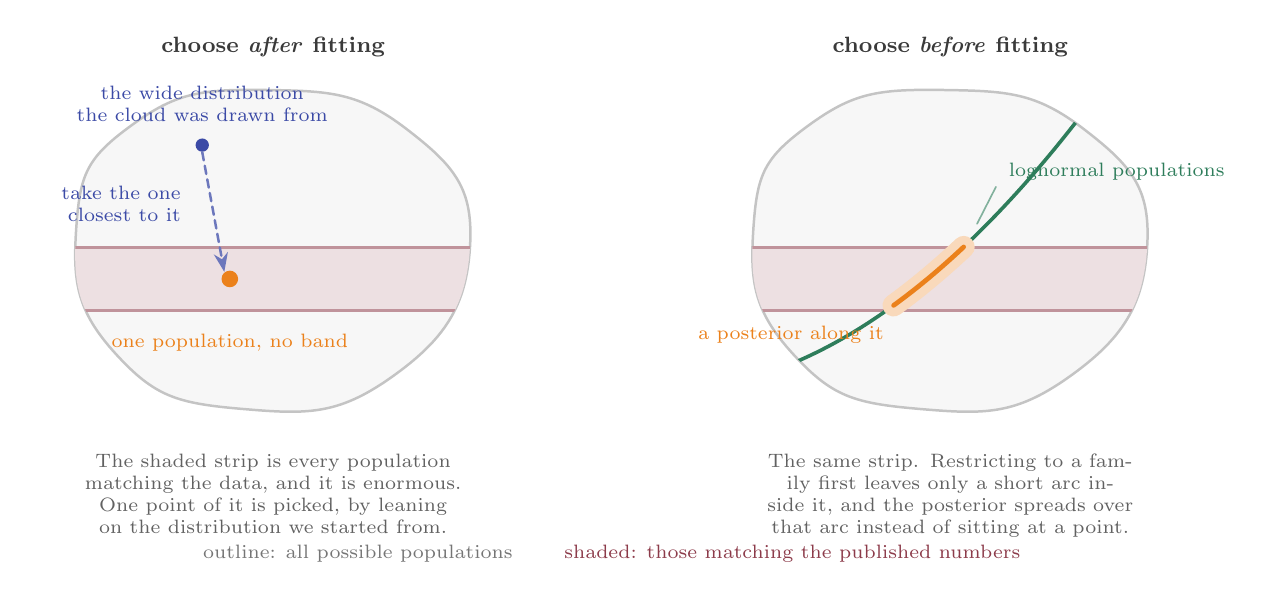
\begin{tikzpicture}[
  font=\sffamily, >=Stealth, line cap=round, line join=round,
  ttl/.style={font=\footnotesize\bfseries, anchor=south},
  figcap/.style={font=\scriptsize, text=ink!80, align=center, anchor=north},
  tag/.style={font=\scriptsize, text=ink!70}]

% ============================================== left: choose after fitting
\begin{scope}[shift={(0,0)}]
  \draw[ink!30, fill=ink!4, line width=0.9pt] \blobpath;
  \begin{scope} \clip \blobpath; \slabfill \end{scope}

  % what the answer is projected from
  \fill[popcol] (-0.9,1.35) circle (2.4pt);
  \node[popcol, font=\scriptsize, anchor=south, align=center] at (-0.9,1.52)
    {the wide distribution\\ the cloud was drawn from};
  \draw[popcol!75, densely dashed, -{Stealth[length=2.4mm]}, line width=0.9pt]
    (-0.9,1.26) -- (-0.62,-0.26);
  \node[popcol, font=\scriptsize, anchor=east, align=right] at (-1.05,0.60)
    {take the one\\ closest to it};

  % the single answer
  \fill[msrcol] (-0.55,-0.35) circle (3pt);
  \node[msrcol, font=\scriptsize, anchor=north] at (-0.55,-0.92)
    {one population, no band};

  \node[ttl, ink] at (0,2.35) {choose \emph{after} fitting};
\end{scope}
\node[figcap, text width=60mm] at (0,-2.45)
  {The shaded strip is every population matching the data, and it is enormous.
   One point of it is picked, by leaning on the distribution we started from.};

% ============================================== right: choose before fitting
\begin{scope}[shift={(8.6,0)}]
  \draw[ink!30, fill=ink!4, line width=0.9pt] \blobpath;
  \begin{scope} \clip \blobpath; \slabfill \end{scope}

  \begin{scope}
    \clip \blobpath;
    % the family: a curve through the same space
    \draw[mechcol, line width=1.3pt]
      plot[domain=-2.4:2.4,samples=90,smooth] (\x,{0.9*\x + 0.12*\x*\x - 0.1});
    % where it crosses the strip: the posterior lives here
    \draw[msrcol!30, line width=8pt]
      plot[domain=-0.72:0.17,samples=30,smooth] (\x,{0.9*\x + 0.12*\x*\x - 0.1});
    \draw[msrcol, line width=1.7pt]
      plot[domain=-0.72:0.17,samples=30,smooth] (\x,{0.9*\x + 0.12*\x*\x - 0.1});
  \end{scope}
  \node[mechcol, font=\scriptsize, anchor=south west] at (0.62,0.78)
    {lognormal populations};
  \draw[mechcol!60, line width=0.6pt] (0.58,0.82) -- (0.34,0.35);
  \node[msrcol, font=\scriptsize, anchor=north east] at (-0.72,-0.82)
    {a posterior along it};

  \node[ttl, ink] at (0,2.35) {choose \emph{before} fitting};
\end{scope}
\node[figcap, text width=60mm] at (8.6,-2.45)
  {The same strip. Restricting to a family first leaves only a short arc inside
   it, and the posterior spreads over that arc instead of sitting at a point.};

% ---------------------------------------------------------------- shared key
\node[tag, anchor=north] at (4.3,-3.60)
  {outline: all possible populations \qquad
   \textcolor{datacol}{shaded: those matching the published numbers}};

\end{tikzpicture}
\end{document}
